\documentclass[aps,prl,onecolumn,reprint,superscriptaddress]{revtex4}
\usepackage{graphicx}
\usepackage{dcolumn}
\usepackage{xcolor}  
\usepackage{comment}
\usepackage{bm}        
\usepackage{amssymb}   % for math
\usepackage{physics}
\usepackage{tikz}
\usepackage{gensymb}
\usepackage{subfigure}
\usepackage{hyperref}
\usepackage{xcolor}
\usepackage{float}
\usepackage{cleveref}
\usepackage{dsfont}
\usepackage{mathtools}
 \usepackage{amsthm}
%\usepackage{kantlipsum} % just to provide mock text

\usepackage[normalem]{ulem}
\newcommand{\mjm}[1]{\textcolor{purple}{#1}}
\newcommand{\mjms}[1]{\textcolor{purple}{\sout{#1}}}
\newcommand{\mjmc}[1]{\textcolor{purple}{\MakeUppercase{#1}}}

\makeatletter
\DeclareRobustCommand{\element}[1]{\@element#1\@nil}
\def\@element#1#2\@nil{%
  #1%
  \if\relax#2\relax\else\MakeLowercase{#2}\fi}
\pdfstringdefDisableCommands{\let\element\@firstofone}
\makeatother
 

\begin{document}
\title{Supplemental Material: Quantum Optimal Control of Nuclear Spin Qudecimals in \textsuperscript{87}Sr}
\author{Sivaprasad Omanakuttan}
\email[]{somanakuttan@unm.edu}
\author{Anupam Mitra}
\affiliation{Center for Quantum Information and Control (CQuIC), Department of Physics and Astronomy, University of New Mexico, Albuquerque, New Mexico 87131, USA}
\author{Michael J. Martin }
\affiliation{Materials Physics and Applications Division, Los Alamos National Laboratory, Los Alamos, New Mexico 87544}
\affiliation{Center for Quantum Information and Control (CQuIC), Department of Physics and Astronomy, University of New Mexico, Albuquerque, New Mexico 87131, USA}
\author{Ivan H Deutsch}
\email[]{ideutsch@unm.edu}
\affiliation{Center for Quantum Information and Control (CQuIC), Department of Physics and Astronomy, University of New Mexico, Albuquerque, New Mexico 87131, USA}
\maketitle

%\section{Open loop Quantum control}

In this supplement we detail the methods we employ for quantum optimal control.  We consider open loop-control to create arbitrary unitary evolution, a problem which is studied extensively in the literature \cite{jurdjevic1972control,brockett1973lie,schirmer2002degrees, goerz2015optimizing, glaser2015training}. In general consider a Hamiltonian in a $d$-dimension Hilbert space of the form, 
\begin{equation}
H(t)=H_0+\sum_{\lambda=1}^{K}c_\lambda(t)H_{\lambda}.
\label{eqn: control Hamiltonian}
\end{equation}
 The system is controllable if we can generate any $U_0\in SU(d)$ using a set of controls $c_\lambda(t)$,  This means that in a finite time $T$, the Hamiltonian evolution given by the Schr{\"o}dinger equation $\dot{U}=-iH(t)U$, maps the identity operator to any arbitrary unitary operator $U_0$ in the group with arbitrary precision. A necessary and sufficient condition for the controllability is the set of Hamiltonians $\{H_0,H_1,H_2,..., H_K\}$ generate the Lie algebra $\mathrm{su}\left(d\right)$.  
 
 In this letter we consider the control of a nuclear spin $\mathbf{I}$ with dimension $d=2I+1=10$ using a combination of radio-frequency driven Larmor precession and a tensor AC-Stark shift according to the Hamiltonian,
\begin{equation}
H(t)=\Omega_{\mathrm{rf}} \left( \cos[c(t) \pi]I_x+\sin[c(t) \pi] I_y\right)+\beta I_z^2.
\label{eq:Control_Hamiltonian}
\end{equation}
It was proved in \cite{Merkel2008} that by manipulating the phase $c(t)$ the above system is controllable.

We consider two classes of quantum control tasks: preparation of a target pure state $\ket{\psi_\text{tar}}$ and implementation of a target unitary map $U_\text{tar}$ on an arbitrary input state.  We implement these tasks using quantum optimal control. The goal is to find the waveform $c(t)$ which optimizes the objective function.  As a first step we discretize the control waveform as a piecewise constant function over $n$ equal intervals in the time $T$, $\mathbf{c}=\{c_i = c(t_i) | i=1,\dots N\}$.  Optimal control for state preparation and unitary maps follows by maximizing the relevant fidelity, 
\begin{eqnarray}
\mathcal{F}_{\psi}[\bm{c},T]&=&\left|\bra{\psi_{\text{tar}}}U[\bm{c},T]\ket{\psi_0}\right|^2,\\
\mathcal{F}_U[\bm{c},T]&=&\left|\Tr\left(U^{\dagger}_{\text{tar}}U[\bm{c},T]\right)\right|^2/d^2.
\label{eq:fidelity}
\end{eqnarray} 
Here $U[\bm{c},T] =\prod_{i=1}^n e^{-iH(c_i)T/n}$.  To find $\mathbf{c}$, we use the well-known gradient based optimization method GRAPE \cite{khaneja2005optimal}. Robust optimization follows when $T$ is sufficiently large compared to the minimal value $T_*$ set by the quantum speed limit~\cite{caneva2009optimal} and $n$ is sufficiently large compared with the minimal number of parameters necessary to specific the control task.  For a $d$-dimensional Hilbert space, $n_{\min} = 2d-2$ for state preparation and $n_{\min} =d^2-1$ for unitary maps.

 %The total time and the number of intervals determine whether the problem is controllable or not; however, an explicit relationship between them is a bigger question and there has been some development in understanding the information theoretical limits of open loop quantum control \cite{lloyd2014information,muller2020information}. 
 
While in principle we can find simple control waveforms with $n$ close to $n_{\min}$, in practice, the resulting discontinuous waveforms may not be exactly realizable in an experimental implementation. To find waveforms that are more experimentally feasible we constrain the maximum jump allowed between $c_i \text{ and } c_{i+1}$ to create a smoother waveform, as was shown in~\cite{Frey2020}.  Another important ingredient is the choice of the initial seed $\mathbf{c}$ to the GRAPE algorithm. A waveform that yields high-fidelity is not unique, and by choosing smoother initial seed, the optimal solution will be smoother as well.    Here we choose the initial condition where $c_i=0 \hspace{0.1cm}\forall i$.  This is sufficiently small so that the time for computer optimization is reasonable, by sufficiently large that we obtain experimentally feasible waveforms, with a maximum of  $c_{i+1}-c_i \leq 0.4 $.  



%\section{Generation of control waveforms with finite bandwidth and slew rate}
While the quantum control technique described above creates relatively smooth waveforms, there still exist discontinuities which can result in a large slew rate and bandwidth that is outside the range of the physical control. To see how this constraint affects the fidelity, we take simple model to pass the phase waveform through a low-pass filter,
\begin{equation}
     c(t)=\phi(t)/\pi=\Omega_c\int_{0}^{t} c_{ideal}(\xi)\exp\left[-\Omega_c(t-\xi)\right]d\xi\\
    \label{eq:LIS}
\end{equation}
where $c_{ideal}(\xi)$ is the ideal waveform value one would attain as the output of the GRAPE algorithm in a perfect piecewise approach. The waveforms depend on the choice of the corner frequency, $\Omega_c$, which is related to the bandwidth of the controller.  Examples of filtered waveforms obtained using $\Omega_c = 20 \Omega_{\rm{rf}} $ are given in Fig.~(\ref{fig:control_waveform_convolution}).  The resulting waveforms are continuous functions of time and band-limited. 

\begin{figure}
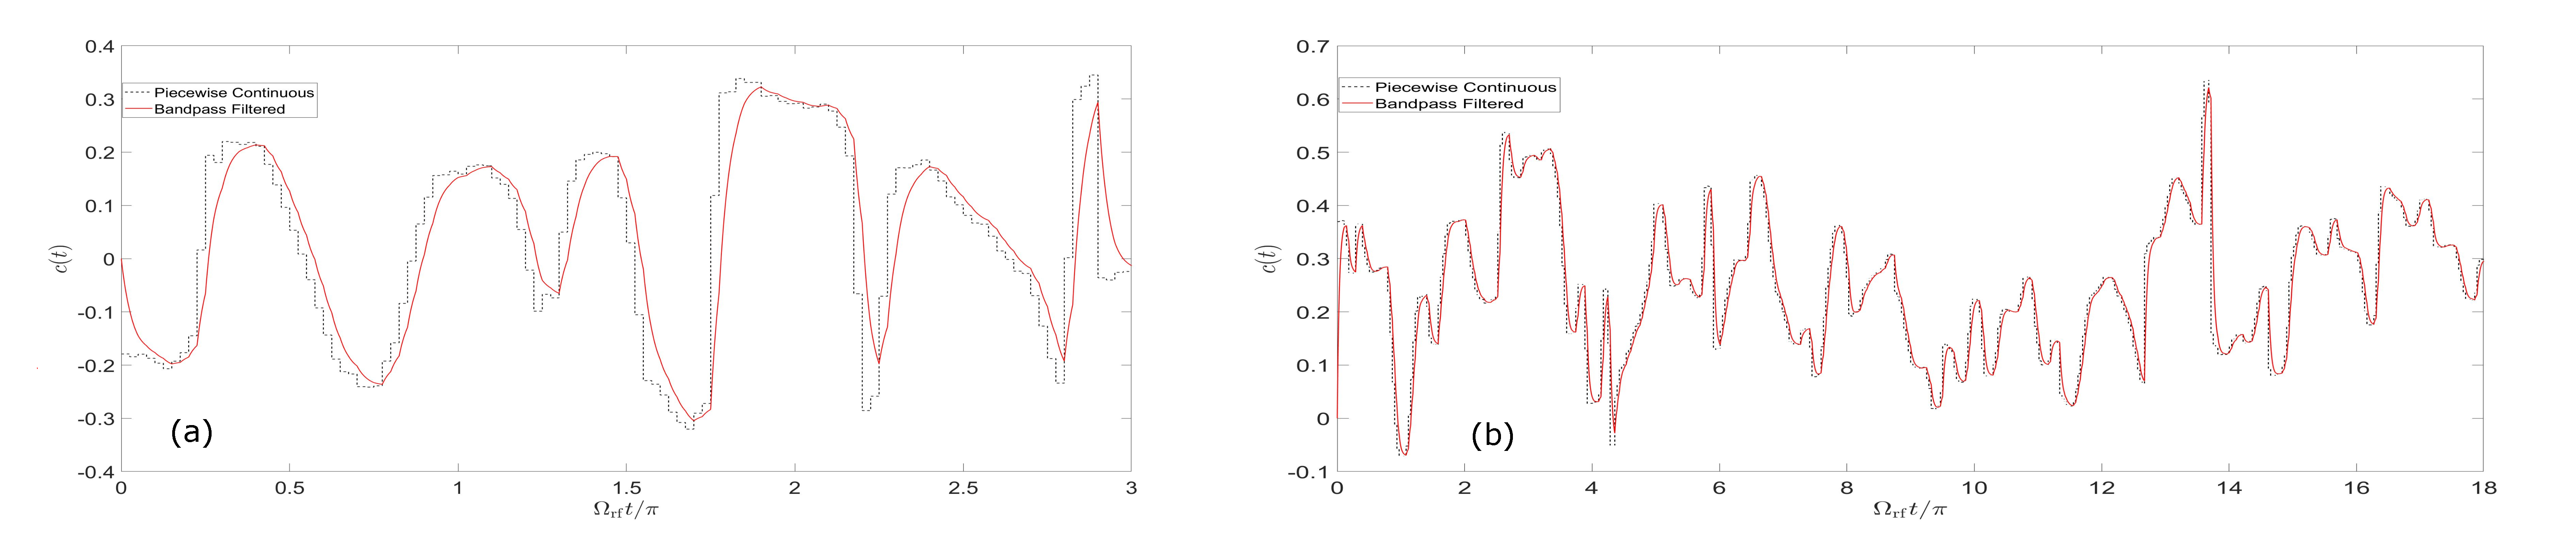
\includegraphics[width=1\textwidth]{band_ramps122.eps}
\caption{Control waveforms for a piecewise constant parameterization, with a limited slew rate (dotted black line) and the waveforms created after the low-pass filter (solid red line ) for the state preparation (a) and unitary mapping (b) with $\Omega_c=10\Omega_{\mathrm{rf}}$.  }
\label{fig:control_waveform_convolution}
\end{figure}

The analysis of the control seed after the low-pass filter shows that there is high fidelity operation can be obtain for $\Omega_c \sim 100 \Omega_{\rm{rf}}$, e.g., $\Omega_{\rm{rf}} = 100$ Hz, $\Omega_{c} = 1$ kHz. The decoherence analysis for the continuous waveforms for the state preparation and  unitary mapping (Eq.(6) and Eq.(7) in the main text)  for $\beta=0.4\Omega_{\mathrm{rf}}$ is given in Fig.~(\ref{fig:control_waveform_convolution_fidleity})

\begin{figure}
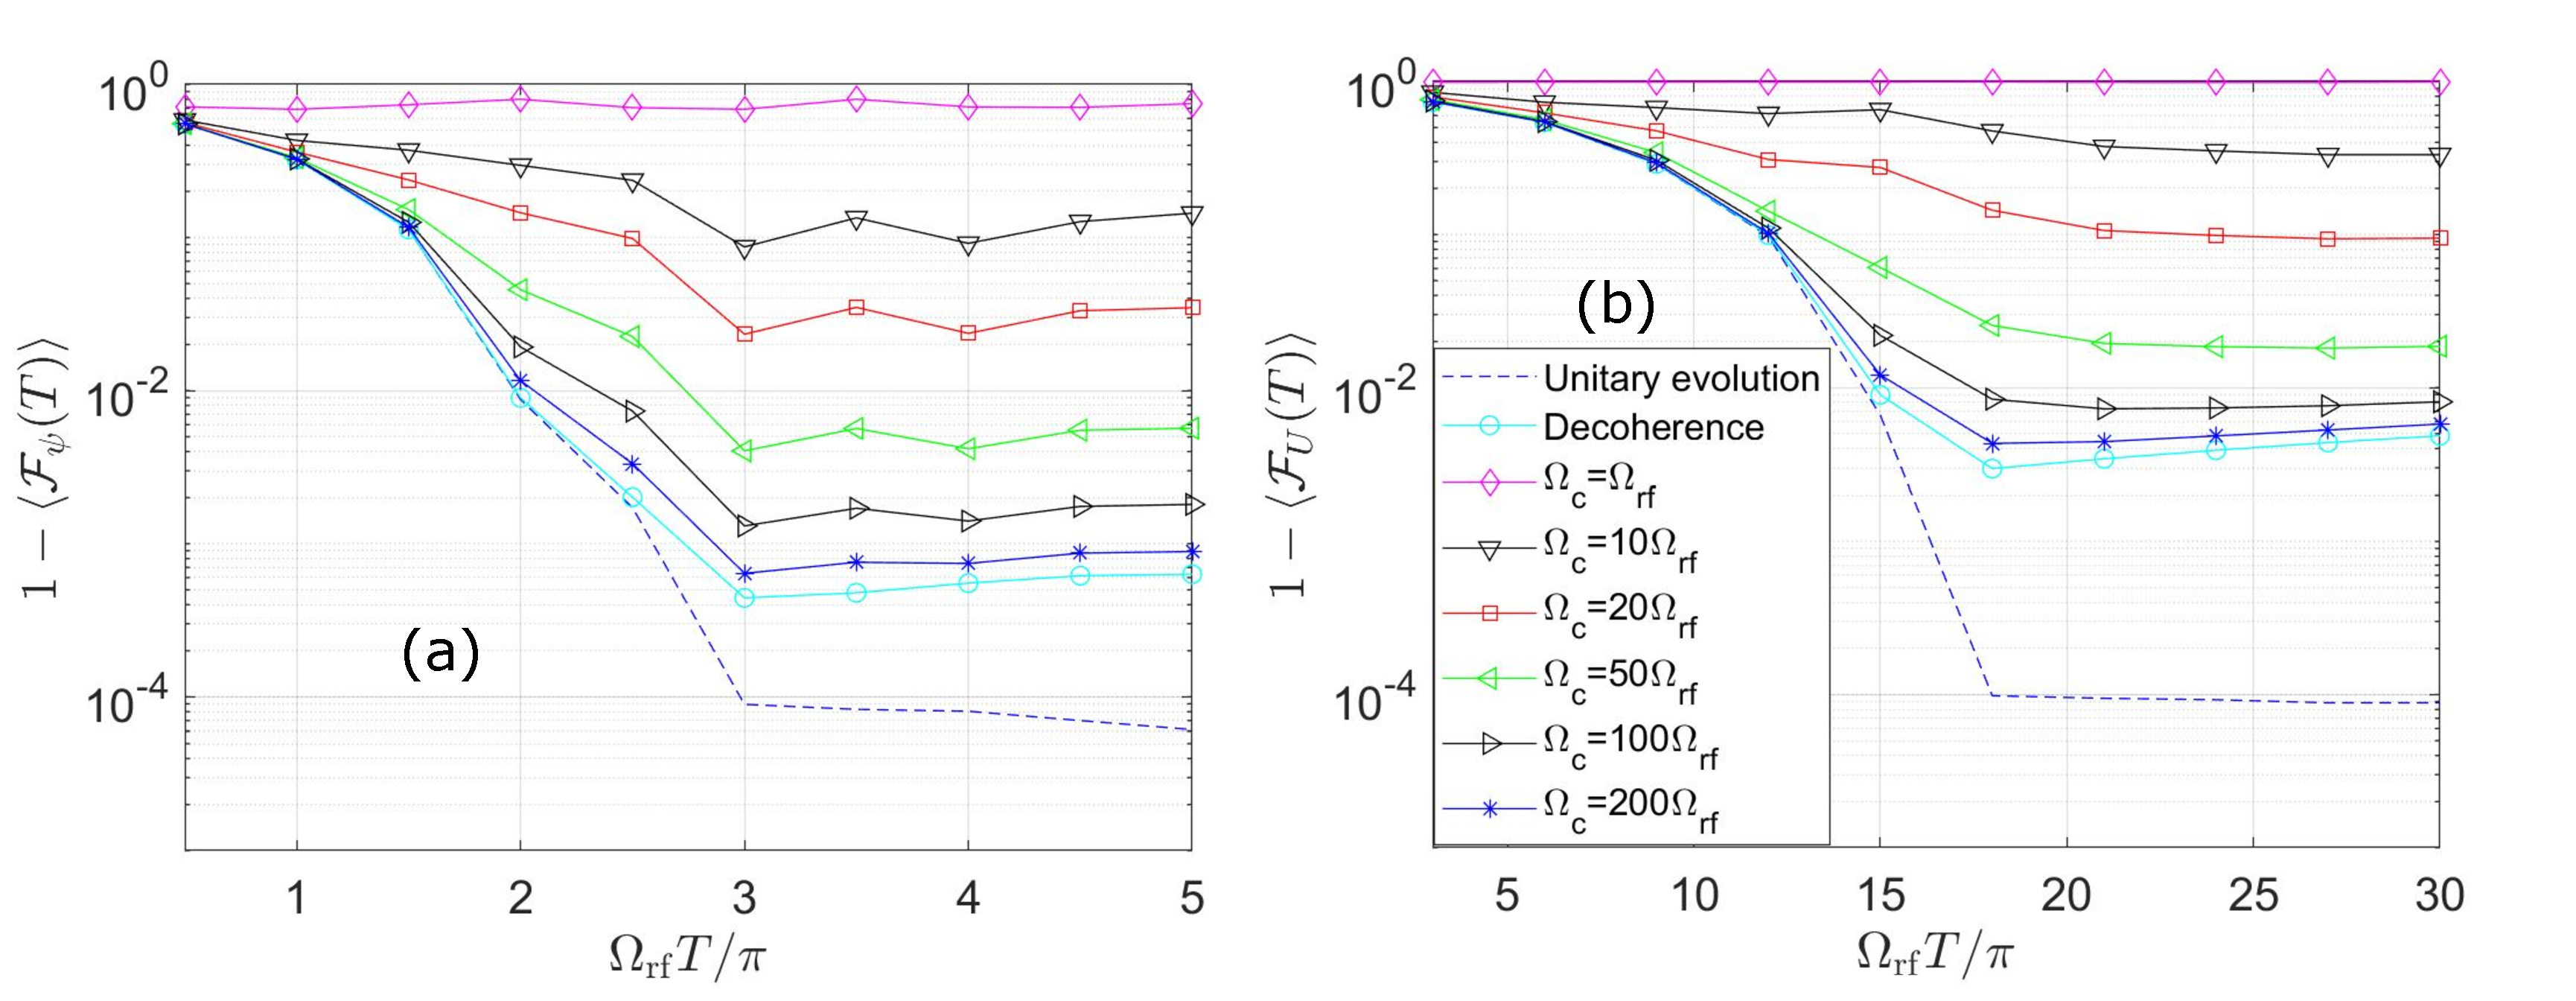
\includegraphics[width=0.8\textwidth]{band_lim.eps}
\caption{The fidelity observed for state preparation (a) and unitary mapping (b) for $\beta=0.4\Omega_{\mathrm{rf}}$ under the full decoherence analysis for different value of the corner frequencey $\Omega_c$.  }
\label{fig:control_waveform_convolution_fidleity}
\end{figure}

\bibliography{reference}
\end{document}